\NextFile{ScoringFunction.html}
\chapter{The MATSim default scoring function (= utility function)}

\authorsOfDoc{Kai Nagel}

\def\betaperf{\beta_{\it perf}}

\begin{chapter-intro}
MATSim contains at its core a co-evolutionary algorithm which continuously generates new alternatives (continuous choice set generation).  The actual choice from that set is based on the scoring function.
\end{chapter-intro}

\begin{note}
What is called ``score'' in MATSim is called ``fitness'' in evolutionary computing and ``utility'' in transport economics.  If you are, say, looking for a mode choice model in MATSim, this is realized by the scoring function (this section) together with the plan selectors (Sec.~\ref{sec:selectors}).
\end{note}

This section contains information that pertains to the so-called ``Charypar-Nagel scoring function''.

In many situations, it should be sufficient to just read Sec.~\ref{sec:quickstart-kn}.  However, if you are working on departure time choice, or related issues such as peak hour pricing, you need to read on beyond that.

\umbruch

\begin{figure}[h]
\centerline{%
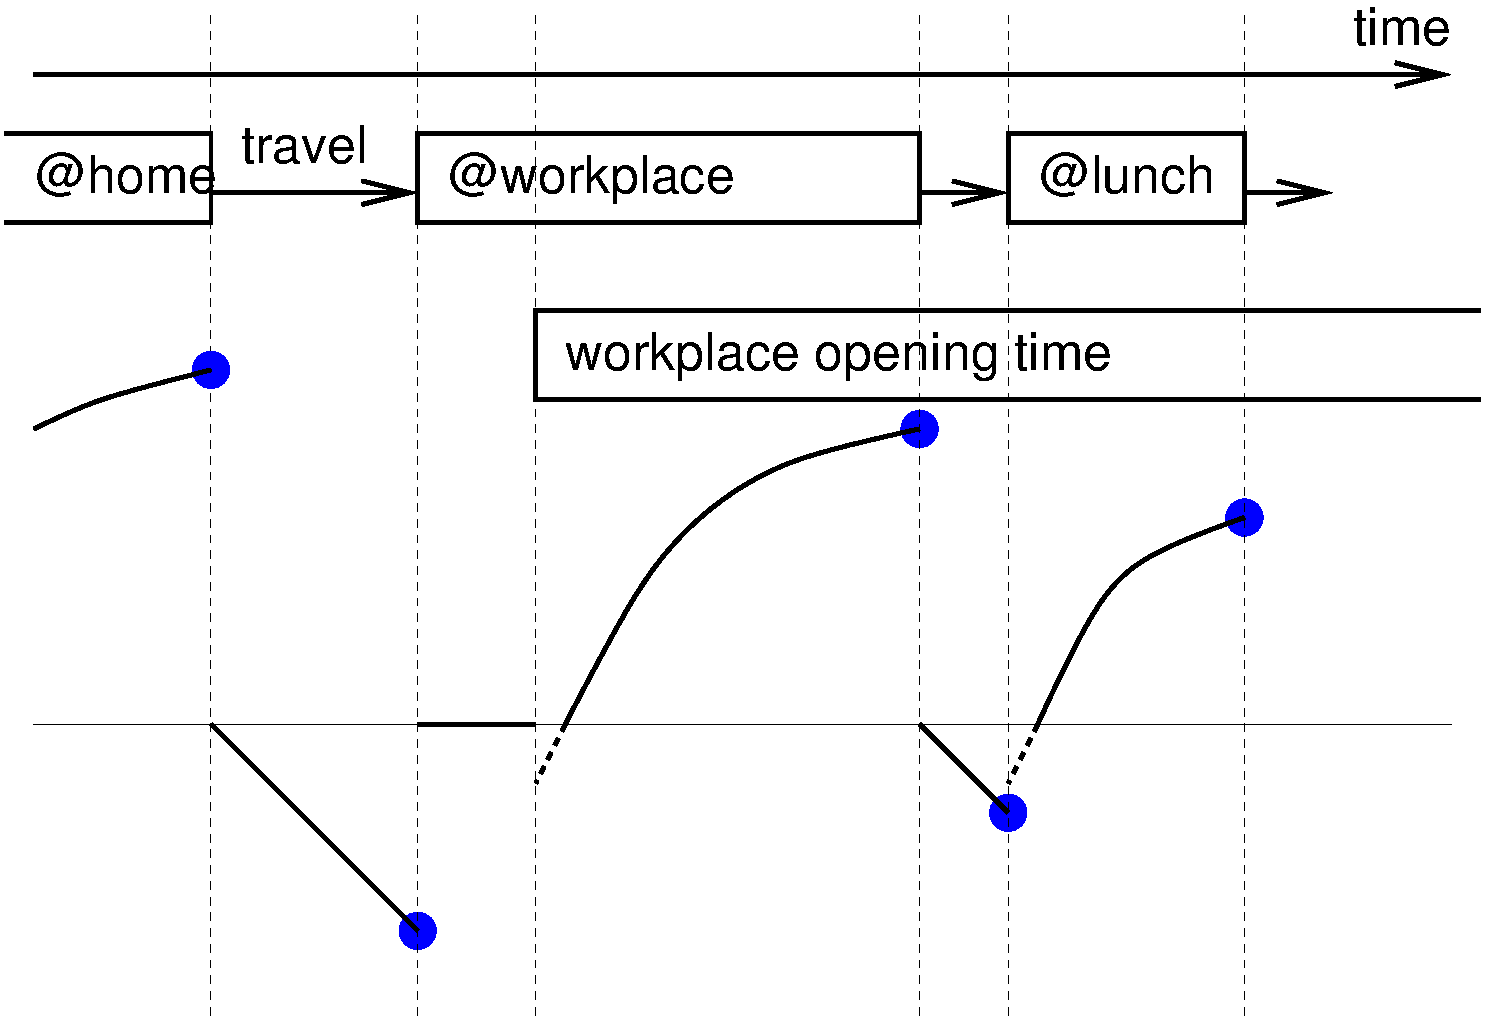
\includegraphics[width=0.6\hsize]{figures/scoringFunction/scoring-example-wo-marginal}
}
\caption{Example of scoring function.}
\label{fig:scoring-example-wo-marginal}
\end{figure}

\section{Illustration}

Synthetic travelers normally receive rewards (positive utility) for performing activities, and penalties (negative utility) for traveling.

Fig.~\ref{fig:scoring-example-wo-marginal} provides an example of a typical scoring function.  
%
Time increases to the right. 
%
The agent first is at home, then travels to the workplace, then travels to lunch, etc.
%
The workplace opening time is different from the time span during which the agent is at the workplace.
%
The distance of the blue dots to the zero line is what the synthetic persons receive at the end of each stage:
\begin{itemize}
\item a positive utility from the ``home'' activity
\item a negative utility from travelling to work
\item ``nothing'' from waiting until the workplace opens
\item a positive utility from the ``work'' activity
\item a negative utility from travelling to lunch
\item etc.
\end{itemize}

One can observe the following:
\begin{itemize}
\item extending an activity increases the utility
\item however, the \emph{marginal} increase of utility \emph{de}creases with increasing utility duration
\item ``doing nothing'' brings neither reward nor penalty
\item travelling incurrs negative utility
\end{itemize}

%% If one looks at the slopes (marginal utilities) at the actual activity durations (Fig.

%% \begin{figure}[h]
%% \centerline{%
%% 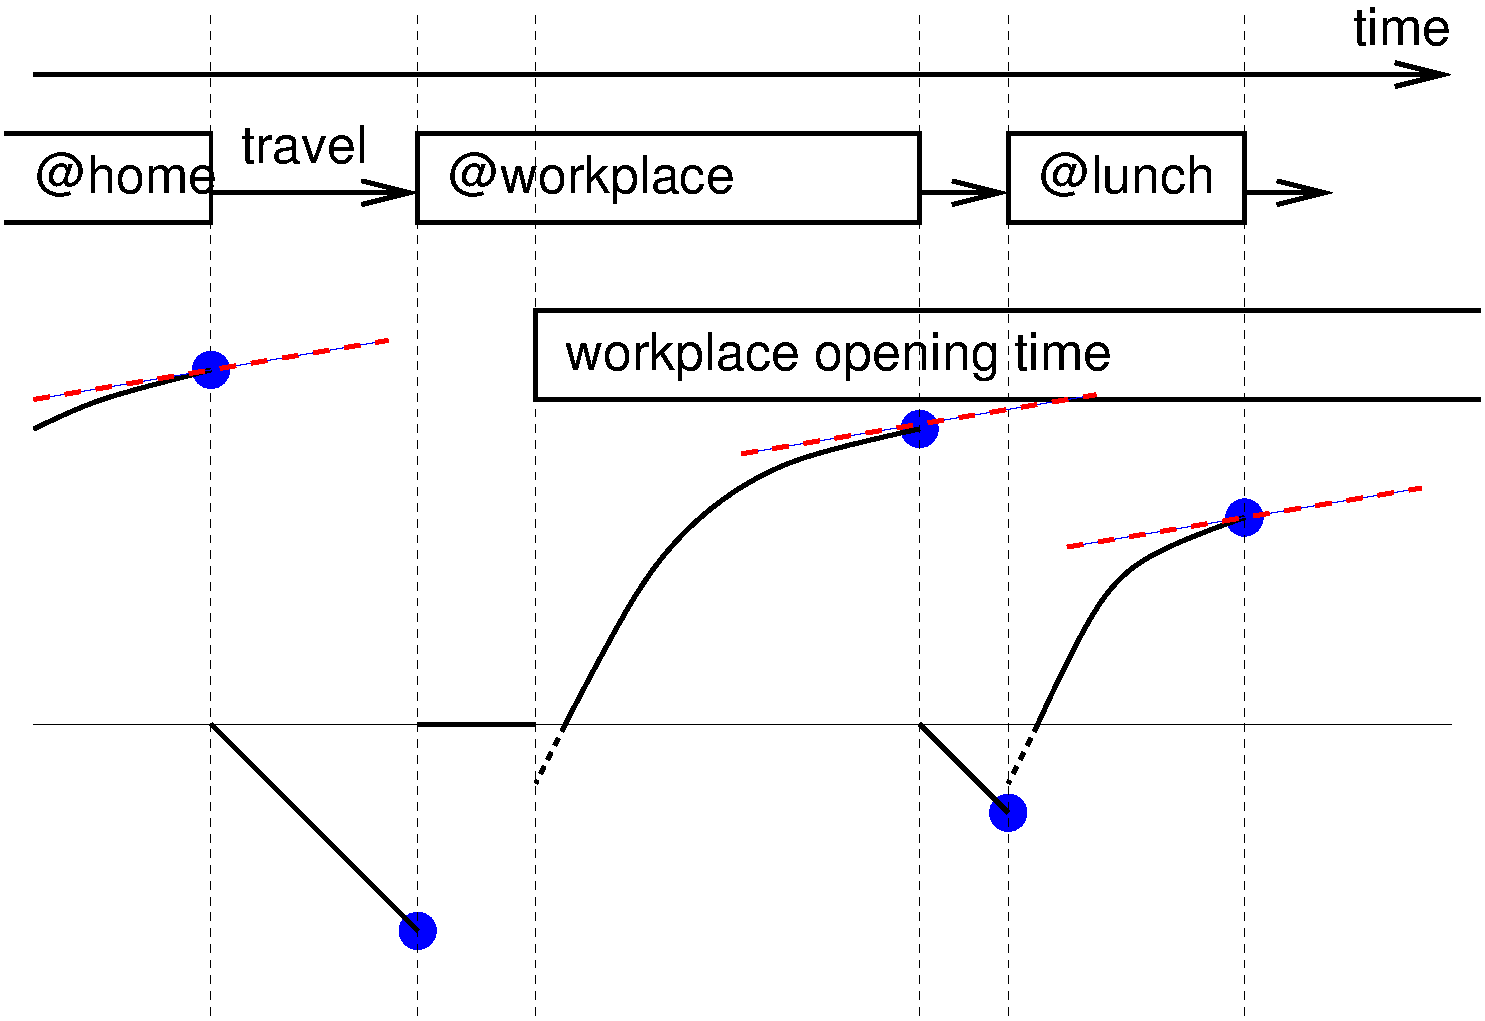
\includegraphics[width=0.6\hsize]{figures/scoringFunction/scoring-example}
%% }
%% \caption{Example of scoring function.}
%% \label{fig:scoring-example}
%% \end{figure}

\section{Mathematical version}

The mathematical version of the scoring function is
\[
V = \sum_i ( V^{perf}_i + V^{late}_i) + \sum_j V^{leg}_j \ .
\]

\subsection{Performing activities}

The (normally positive) reward of performing activity $i$ is
\[
V^{perf}_i = \beta_{perf} \cdot t_{typ,i} \cdot \ln( t_{perf} / t_{0,i} ) 
%
\qquad \mbox{ for } \qquad
%
t_{perf} \ge t_{0,i} \ ,
\]
where
\begin{itemize}

\item
$t_{perf}$ is how long the agent performed the activity, 

\item $t_{typ,i}$ is its typical duration (e.g.\ 8~hours for ``work'', 12~hours for ``home''), and

\item $\beta_{perf}$ is a slope.

\item  $t_{0,i}$ is more confusing than it looks, and has less influence than one may think, and therefore we ignore it for the time being.

\end{itemize}

\subsection{Arriving late}

The (normally negative) penalty of arriving late is
\[
V^{late}_i = \beta_{late} \cdot t_{late} \ ,
\]
where $t_{late}$ is the amount of time the agent arrived late, and $\beta_{late}$ is a (normally negative) slope.

\subsection{Traveling}

The (normally negative) penalty of traveling is
\[
V^{leg}_j = \beta_{trav,mode} \cdot t_{trav} 
%
+ \beta_m \cdot m_{trav}
%
+ (\beta_{dist,mode} + \beta_m \cdot \gamma_{dist,mode}) \cdot d_{trav}
%
+ V_{transfer}
\]
where
\begin{itemize}
\item $t_{trav}$ is the time spent traveling
\item $\beta_{trav,mode}$ is a (normally negative or zero, see below) slope
\item $m_{trav}$ is the change of the monetary position caused by the travel (normally negative, e.g.\ a toll or a fare)
\item $\beta_m$ is a (normally positive) slope; this is the marginal utility of money
\item $d_{trav}$ is the distance of the leg
\item $\beta_{dist,mode}$ is a (normally negative) slope
\item $\gamma_{dist,mode}$ is a (normally negative) distance cost rate
\item $V_{transfer}$ is a transfer penalty e.g.\ incurred in public transit systems
\end{itemize}
The negative effects of distance can be included both directly as a marginal disutility and indirectly as a distance cost rate.  The first is presumably more applicable for a mode with mostly physical exercise, such as walk, whereas the latter is presumably more applicable for a mechanical mode, such as car.  Bicycle may incur both.

The notation deliberately uses ``leg'' and not trip, since this allows to decompose a trip into multiple legs, all with separate scoring contributions.

\subsection{Utility of time as a resource (opportunity cost of time)}
\label{sec:utl-of-time-as-resource}

Most utility-based models in travel behavior research, such as typical logit mode choice models, use partial utility functions: These utility functions do not describe the full utility of the person, but just those parts that are affected by the choice.

Since MATSim gives a score/utility to the full day, this does not work in the same way any more.  It most importantly shows up with time, where reducing the time spent traveling does not only lead to a reduction of the penalty of traveling, but also (barring opening time constraints) to an extension of the activity following the travel.

The first effect is described marginally by
\[
- \frac{\partial}{\partial t_{trav}} V^{leg} = - \beta_{trav,mode} \ ,
\]
the minus stems from the fact that we are \emph{reducing} the travel time.

The second effect is described marginally by
\[
\frac{\partial}{\partial t_{perf}} V^{perf}_i
%
= \beta_{perf} \cdot t_{typ,i} \cdot \frac{1}{t_{perf}}
%
\approx \beta_{perf} \ ,
\]
where the approximation holds when the actual activity duration $t_{perf}$ is close to its typical duration, $t_{typ,i}$.  This is also the justification why $t_{typ,i}$ is called the typcical duration, and $\beta_{perf}$ the marginal utility of performing.

The marginal utility of travel time savings needs to consider both:
\[
mUTTS 
%
= \left( - \beta_{trav,mode} + \beta_{perf} \cdot \frac{t_{typ,i}}{t_{perf}} \right)
%
\approx - \beta_{trav,mode} + \beta_{perf} \ .
\]
In consequence, $\beta_{trav,mode}$ \myemph{is only an offset to the marginal utility of time as a resource}.  If travelling is considered more pleasant than ``doing nothing'', it may actually be positive.  Even when it is positive, the overall marginal utility of travel time ($= -mUTTS$) can still remain negative.

The better known (marginal) value of travel time savings is obtained by dividing these values by the marginal utility of money:
\[
VTTS = \frac{mUTTS}{\beta_m} 
%
= \frac{\left( \beta_{perf} \cdot \frac{t_{typ,i}}{t_{perf}} - \beta_{trav,mode} \right)}{\beta_m}
%
\approx \frac{\beta_{perf} - \beta_{trav,mode}}{\beta_m} \ .
\]



\section{Calibration of the scoring function}

%% \subsection{Quickstart}
\label{sec:quickstart-kn}

A possible approach is as follows:\footnote{%
%
Different groups have different systems, this is mine, although I took ideas from Michael Balmer.
%
}
\begin{enumerate}

\item Set $\beta_{scale} \equiv$ \verb$BrainExpBeta$ to $1.0$.  (This is the default.)

This is normally a positive value.

\item Set $\beta_{money} \equiv$ \verb$marginalUtilityOfMoney$ to whatever is the prefactor of your monetary term in your mode choice logit model.

If you do not have a mode choice logit model, set to $1.0$. 

This is normally a positive value (since having more money normally increases utility).

\item Set $\betaperf \equiv$ \verb$performing$ to whatever is the prefactor of car travel time in your mode choice mode (probably with a sign change, see below).

If you do not have a mode choice logit model, set to $+6.0$.

This is normally a positive value (since performing an activity for more time normally increases utility).

\item Set $\beta_{tt,car} \equiv$ \verb$traveling$ to $0.0$.

\myemph{It is important to understand this:}  Even if this value is set to zero, traveling by car will be implicitly punished by the so-called opportunity cost of time: If you are traveling by car, you cannot perform an activity, and thus you are (marginally) losing $\betaperf$.  Sometimes also called the ``utility of time as a resource''.

\item Set all other marginal utilities of travel time by mode \myemph{relative to the car value}.

E.g.\ if your logit model says something like 
\[
... -6/h \cdot tt_{car} - 7/h \cdot tt_{pt} ... ,
\]
then 
\[
\betaperf = 6 \ , \ \ \beta_{tt,car} = 0 \ , \hbox{ and } \beta_{tt,pt} = -1 \ .
\]

If you do not have a mode choice logit model, set all $\beta_{tt,mode} \equiv$ \verb$travelingXxx$ values to zero (i.e.\ same as car).

\item Set the distance cost rates \verb$monetaryDistanceCostRateXxx$ to plausible values if you have them.

For the time being, this needs to be negative (which is not entirely plausible but it is the way it is).

\item Use the alternative-specific constants $C_{mode} \equiv$ \verb$constantXxx$ to calibrate your modal split.

(This is, however, not completely simple: One needs to run iterations and look at their end, and especially for modes with small shares one needs to have innovation switched off early enough near the end of the iterations.)

\end{enumerate}

If you end up having your modal split right but its distance distribution not, you probably need to look at the different mode speeds.  In our experience this works better than using the $\beta_{tt,mode}$ for this.

Calibrating schedule-based pt currently goes beyond what can be provided here; recommendations:
\begin{itemize}

\item Stay away from schedule-based pt until you really understand what you are doing.

\item Treat schedule-based pt as a ``mechanical'' model which just transports people.  For this, completely switch off mode choice.

\item Make a support contract with senozon.

\item Write a joint funding proposal with the MATSim group in Berlin (or in Zurich, but I haven't asked them).  This needs to provide funding for us that is large enough to do research and not just support.

\end{itemize}

%% \subsection{Some explanation: Simplified version}
%% \label{sec:some-expl-simpl}

%% The simplified version assumes that all activities operate near their typical duration. In this case (see \href{http://matsim.org/node/651}{here}),  one can approximate the marginal utility of activity duration (i.e. the  marginal utility if the sum of all activities is extended by that  amount of time) by $\betaperf$.

%% Now let us consider the typical changes (of the Vickrey  scenario). Note that in the Vickrey scenario, the meaning of the  marginal utility of arriving earlier means the marginal contribution  assuming that the travel time remains the same. We will assume  that activities are ended by the endtime attribute, not by the duration  attribute.

%% \subsubsection{Travel takes longer (by amount $\Delta t$)}

%% In this situation, the activity that follows the trip is cut short by  $\Delta t$. We thus have the following (linearized) modifications  of the utility:
%% \begin{itemize}

%% \item Travel takes longer by $\Delta t$; the utility change is  $\beta_{tt} \cdot \Delta t$. Note that $\beta_{tt}$ typically is  negative.

%% \item The following activity is shortened by $\Delta t$; the (linearized)  utility change is $- \betaperf \cdot \Delta t$.  $\betaperf$ is  typically positive, so the contribution is negative.

%% \end{itemize}
%% Overall: The (linearized) utility change caused by longer travel is
%% \[
%% ( - \betaperf + \beta_{tt} ) \cdot \Delta t \ .
%% \]


%% \subsubsection{Traveller increases arriving early (by amount $\Delta t$)}

%% In this situation, the traveller will ``do nothing'' between the  arrival and the opening time of the activity. That is, the amount  of time that the traveller is doing nothing is now increased by  $\Delta t$. Consistent with the meaning of the Vickrey parameter  ``marginal utility of arriving early'', we assume that the travel time is  the same compared to the later arrival. This means that the preceeding  activity was cut shorter by $\Delta t$. We thus have the following  (linearized) modifications of the utility:
%% \begin{itemize}

%% \item The preceeding activity is shortened by $\Delta t$; the
%% (linearized) utility change is $- \betaperf \cdot \Delta t$.
%% 	$\betaperf$ is typically positive, so the contribution is
%% 	negative.

%% \end{itemize}
%% There are no other contributions, since the time between the  arrival and the opening time prodices neither positive nor negative  utility contributions. Overall: The (linearized) utility change  caused by arriving early is
%% \[
%% - \betaperf \cdot \Delta t \ .
%% \]
%% That is, as long as there are no  additional utilities or disutilities of waiting, the marginal utility of  performing can be approximated by the marginal utility of schedule  delay early.

%% \subsubsection{Traveller increases arriving late (by amount $\Delta t$)}

%% In this situation, we have the following (linearized) modifications of the utility:
%% \begin{itemize}

%% \item The preceeding activity is extended by $\Delta t$; the
%% (linearized) utility change is $\betaperf \cdot \Delta
%% t$. $\betaperf$ is typically positive, so the contribution is
%% positive.

%% \item The following activity is shortened by $\Delta t$; the (linearized)  utility change is $- \betaperf \cdot \Delta t$. $\betaperf$ is  typically positive, so the contribution is negative (and exactly cancels  the previous contribution).

%% \item Arriving late is increased by $\Delta t$; the (exact) utility change  is $\beta_{late} \cdot \Delta t$. $\beta_{late}$ is typically negative, so  the contribution is negative.

%% \end{itemize}

%% Overall: The (linearized) utility change caused by increasing the amount of arriving late is
%% \[
%% \beta_{late} \cdot \Delta t \ .
%% \]


% this is already said above (in quickstart)
%%\subsubsection{Overall}

%%Overall, calibration of the Charypar-Nagel scoring function is best done as follows:
%%\begin{itemize}
%%	\item \textbf{Run a survey and estimate logit models that include  penalties for travelling (by mode), schedule delay early, and schedule  delay late.}
%%	\item \textbf{The marginal utility of schedule delay early from the logit  model, multiplied by minus one, results in the MATSim beta\_perf.}  Since the marginal utility of schedule delay early is typically  negative, beta\_perf is thus typically positive. This is the  marginal opportunity cost of time. A useful interpretation is that  this is the difference between "leisure" and "doing nothing".
%%	\item \textbf{The marginal utility of travelling from the logit model, \emph{plus beta\_perf,} results in the MATSim beta\_trav (by mode).} That is, the MATSim beta\_trav is an \emph{additional utility offset}  when compared to doing nothing. Since driving can well be seen as  more positive than doing nothing (e.g. because of making phone calls,  listening to music, enjoying to drive), the MATSim beta\_trav can well be  positive.
%%\\   (Note that this has still nothing to do with "positive values of  travel time", e.g. by Susan Handy. Those positive values imply  that the additional utility offset over-compensates the marginal  opportunity cost of time. In other words, "time spent driving  home" is (to an extent) seen more positive than "being at home".)
%%	\item \textbf{The marginal utility of being late from the logit model results in the MATSim beta\_late.}
%%	\item Note that you also need reasonable values for opening time, latest  arrival time, and closing time, in order to achieve that the schedule  delay cost mechanics works in MATSim. This is quite clear if you  think about it; nevertheless, it has been forgotten uncountable times  (in particular in studies that start from trips, not from full daily  plans).
%%\end{itemize}

%% \subsection{Without schedule delay}

%% If you intend to run MATSim without time adaptation  (TimeAllocationMutator), these things are not that critical. In  that situation, you just need to make sure that $\betaperf + \beta_{tt}$  matches your marginal utility of travel time savings. An easy  way in our view is:
%% \begin{itemize}

%% \item Set $\beta_{tt,car}$ to zero (i.e.\ assume that driving
%% 	is as good or bad as doing nothing).  

%% \item Set $\betaperf$ to
%% 	the estimated marginal utility of travel time savings (make
%% 	sure you get the sign right; $\betaperf$ should be
%% 	positive).  \item Set (say) $\beta_{tt,pt}$ to your estimated
%% 	marginal utility of travel time savings (should be
%% 	positive) \emph{minus} the MATSim $\betaperf$. The result may
%% 	be positive (implying that spending time using the mode is
%% 	better than doing nothing) or negative (implying that spending
%% 	time using the mode is worse than doing nothing).
%% \end{itemize}
%% Note that even without time adaptation, $\beta_{late}$ may still have an influence if you have set the latest arrival times for some  activities.

%% \subsection{Full version}

%% ``Full version'' would imply that we could calibrate the MATSim  parameters also for situations where the actual activity durations are  far from their ``typical'' values. This could happen for two reaons:
%% \begin{itemize}

%% \item There are too many activities that need to be squeezed into a  day. A possible interpretation would be that $\betaperf$ corresponds  to the marginal utility of additional leisure time on, say, sundays,  but the weekday activites cannot be shifted to sundays.

%% \item There are too many activities that need to be squeezed
%% into certain time periods, say between day care opening and closing,
%% or into typical business hours.

%% \end{itemize}
%% Both of these interpretations make sense (in my view) and should be
%% investigated for MATSim. Presumably, there is already general
%% research; it would then be necessary to bring that research and the
%% MATSim formulation together.


\section{Default values for the Charypar-Nagel scoring function}

As explained \href{http://matsim.org/node/650}{here},  the MATSim scoring function has, under some circumstances (actual  durations near "typical" durations"), some similarity to the Vickrey  scenario.

The "typical" parameters of the Vickrey scenario are 
\[
\hat\beta_{early}=-6~,~~\hat\beta_{travel}=-12~\mbox{, and } \hat\beta_{late}=-18 \ .
\]

For MATSim, as explained in Sec.~\ref{sec:utl-of-time-as-resource}, %Sec.~\ref{sec:some-expl-simpl}, 
this translates into
\[
\betaperf=6~,~~\beta_{travel}=-6\mbox{ , and } \beta_{late}=-18 \ . 
\]
These are the parameters that were, for a lack of  estimated parameters, introduced into (the precursor of) MATSim  approximately in 2006.

These parameters are multiplied with the beta\_brain parameter, which  can be seen as a separately configurable logit scale parameter. A  useful setting for this parameter was determined via systematic tests  concerning the stability of the iterations, see \href{https://svn.vsp.tu-berlin.de/repos/public-svn/publications/vspwp/2004/04-03/}{here}.

As a next step, an infrastructure to compare MATSim simulations with  real world traffic counts was set up. Only after that  infrastructure was there, an attempt to calibrate the MATSim parameters  from a survey was made. This is documented \href{https://svn.vsp.tu-berlin.de/repos/public-svn/publications/vspwp/2009/09-10/}{here}, unfortunately in German. Two results were
\begin{itemize}
	\item The estimated parameters all have the same order of magnitude as the MATSim default parameters (the "Vickrey" parameters).
	\item The results with respect to traffic counts were not considerably different from before.
\end{itemize}



\section{Interpretation of the logarithmic "utility of performing"}

The  so-called "Charypar-Nagel scoring function" is used in many  MATSim  studies. It is called that way because there is an ancient paper   where this scoring function was introduced.

It uses a logarithmic utility of time for activities: $U = \beta \cdot t_{typ} \cdot  \ln(x/t_0)$ . I sometimes call $t_{typ}$ the ``typical duration''.

The first derivative of U is beta at the typical duration:
\begin{itemize}
	\item 
$\displaystyle
\frac{dU}{dx} = \beta \cdot t_{typ} / x
$
	\item 
$\displaystyle
\left. \frac{dU}{dx}\right|_{x=t_{typ}} = \beta
$
\end{itemize}

Interpretation: marginal utility of duration at "typical duration" is indep of activity type. (*)

The second derivative of U at the typical duration is
\begin{itemize}
	\item 
$\displaystyle
\frac{d^2U}{dx^2} = - \beta \cdot t_{typ} / x^2
$
	\item 
$\displaystyle
\left. \frac{d^2U}{dx^2} \right|_{x=t_{typ}} = - \beta / t_{typ}
$
\end{itemize}

An  important consequence of this is that there is no separate  free  parameter to calibrate the curvature (= 2nd derivative) at the  typical  duration: $\beta$ needs to be the same across all activities, and  $t_{typ}$ is  given by (*).

A second consequence is that $t_0$ is largely  irrelevant. It  shifts the function up and down, i.e.\ it determines how  much you lose  if you drop an activity completely.

In the  original paper (and in most of MATSim), $t_0$ is set to $t_{typ} \cdot   \exp(-10h/t_{typ})$ . This has the (intended) consequence that all  activities  have the same utility contribution at their typical  duration:
\[
U = \beta \cdot t_{typ} \cdot \ln( x / t_{typ} / \exp(-10h/t_{typ}) ) 
%
= \beta \cdot t_{typ} \cdot [ \ln( x/t_{typ} ) + 10h/t_{typ} ]
\]
which   is, at $x=t_{typ}$,
\[
= \beta \cdot t_{typ} \cdot [ 0 + 10h/t_{typ} ] = \beta \cdot  10h \ . 
\]
With  our usual $\beta = 6Eu/h$, this results in $60Eu$ per  activity.

The slope at $U=0$, i.e.\ at $x=t_0$, is
\[
(\beta \cdot t_{typ} / t_{typ}) \cdot \exp( 10h/t_{typ}) = \beta \cdot \exp( 10h/t_{typ} )
\]
which \emph{de}creases with increasing $t_{typ}$. This means that activities with larger typical duration are \emph{easier} to drop completely.

In the end, this makes sense: Since the additional score of any activity is the same, the score \emph{per time} is smallest for activities with long typical durations. Therefore, it makes sense to drop them first.

But practically, this is probably not desired behavior, since it would first drop the home activity from a daily plan.

Overall, therefore: \myemph{In my opinion, the current utility function does not work for activity dropping.}

---

An  alternative, never tested since activity dropping was never  tested with  this utl fct, would be to recognize that $U'(t_0) = \beta \cdot  t_{typ} / t_0$ ,  i.e.\ \emph{increasing} \emph{slope} with \emph{decreasing}  $t_0$.  That is, high priority activities should have $t_0$ such that  $t_{typ}/t_0$ is  large (large slope = hard to drop). Activities of the  same priority  should have $t_0$ such that $t_{typ}/t_0$ is the same between  those activities.  Overall, something like
\[
weight \propto t_{typ}/t_0
\]
or
\[
t_0 \propto t_{typ}/weight
\]
where large weight implies a large importance of the activity.

This  was, as said, never tried, since activity dropping was never   systematically tried. It also does not fix the problem, discussed   later, that different activities might have different resistance  against  making them shorter; since this is U'', this is -beta/t\_x  with the  above utl fct: activities are shortened proportional to their  typical  duration.

---

\st{To make matters worse, there is currently the  convention that  negative values of U are set to zero. This is done  since we need  useable values for negative durations (since they may  happen at the  "stitching together" of the last to the first activity of a  day), and  if we give those a "very negative" score, then the utl at t=0  cannot be  even smaller than this.}

\st{This has, however, the  unfortunate consequence that the ``drift  direction'' of the adaptive  algorithm, once an activity duration has  gone below $t_0$, goes to zero  duration.}

The above was modified in nov'13, see \url{https://matsim.atlassian.net/browse/MATSIM-191}.  It now takes the slope at $t=t_0$ and extends it with that slope to the left.

\section{Outlook}

Outlook: What would we want for our next generation utl function? Some wishes from my perspective:
\begin{itemize}
	\item Curvature at typical duration can be calibrated
	\item Slope at $U=0$ can be calibrated
	\item Utl function extends in meaningful way to negative durations (this would fix the arbitrary handling that we currently employ)
\end{itemize}

In  my view, a polynomial of second degree would be worth trying.\footnote{%
%
As  usual,  there are several ways to set this up. One way is to  expand around the  typical duration:
\[
U(t_{typ} + \epsilon) = U(t_{typ}) + \epsilon \cdot U'(t_{typ}) + \epsilon^2 * U''(t_{typ})/2
\]
or
\[
U(x) = U(t_{typ}) + (x-t_{typ}) \cdot U'(t_{typ}) + (x-t_{typ})^2 * U''(t_{typ})/2
\]
with $t_{typ} =$ typical duration, $U'(t_{typ}) = \beta =$ marg utl at typ dur, $U''(t_{typ}) =$  curvature at typ dur (``priority''), and $U(t\_x) =$ ``base value of act'' (which could be something like $\beta \cdot t_{typ}$ ).
\\
---
\\
Another way (having the parabola going through (0,0)) would be
\[
U(x) = - a x ( x - c ) = - a x^2 + a c x
\]
\[
U'(x) = - 2 a x + a c
\]
\[
prio = U'(x=0) = a c , i.e.\ c = prio/a .
\]
\[
\beta = U'(x=t_{typ}) = - 2 a t_{typ} + prio \hbox{, i.e.\ } a = (prio - \beta)/2t_{typ}
\]
}

There is other work (e.g. by Joh) that should be looked at.

% Local Variables:
% mode: latex
% mode: reftex
% mode: visual-line
% TeX-master: "../user-guide.tex"
% comment-padding: 1
% fill-column: 9999
% End: 
